\chapter{Introducción}
\label{cap:introduccion}



%-------------------------------------------------------------------
\section{Motivación}
%-------------------------------------------------------------------
\label{cap:sec:motivacion}

Hoy en día, el español es la segunda lengua más hablada del mundo y actualmente más de 90.000 palabras forman el castellano. 
Se trata de una lengua con multitud de términos, y que dependiendo del contexto en el que se encuentren, pueden tener múltiples significados. Por ejemplo, la palabra gato puede hacer referencia a un animal o a una herramienta para elevar un coche.
Si esto supone una complicación para cualquier persona, para ciertos colectivos afectados por algún trastorno cognitivo lo es aún mucho más, afectándoles en su vida cotidiana, profesional o personal. Por ejemplo, el simple hecho de leer un periódico es una acción bastante difícil para ellos ya que muchas palabras no saben lo que significan. Otro ejemplo podría ser leer un manual de instrucciones, donde se encuentran en la misma situación de no poder entender ciertos conceptos.

Una de las soluciones que se podrían pensar en un primer momento, es buscar su significado en un diccionario. Pero esto no les sirve, puesto que las definiciones que aparecen en muchos casos no utilizan términos o frases sencillas. Por ejemplo, la palabra computadora tiene la siguiente definición en el diccionario: 
\textit{Máquina electrónica que, mediante determinados programas, permite almacenar y tratar información, y resolver problemas de diversa índole}\footnote{https://dle.rae.es/?id=A4hIGQC}. 
Esta definición puede ser bastante complicada de entender por alguna persona con discapacidad cognitiva ya que utiliza términos más técnicos y es una frase bastante larga. La solución que se ha pensado para poder solventar dicho problema, es ofrecer una definición que compare el concepto en cuestión con otros conceptos más sencillos ya conocidos por el usuario. Para hacer estas comparaciones usaremos las figuras retóricas, más concretamente haremos uso de metáforas, analogías y símiles.
Por ejemplo, para la palabra computadora se podrían obtener los siguientes resultados:
\begin{itemize}
	\item Metáfora: \textit{Una computadora es un ordenador}.
	\item Analogía: \textit{Una computadora es como una máquina}.
	\item Símil: \textit{Una computadora es fuerte como una piedra}.
\end{itemize}

Creemos que el uso de las figuras retóricas facilitará el entendimiento del concepto. En estas definiciones se utilizarán frases cortas y conceptos sencillos. 
Además, añadiremos pictogramas a los resultados para llegar a un colectivo más amplio.

Por tanto, lo que proponemos es crear una aplicación que dada una palabra compleja devuelva una definición de la palabra mediante comparaciones con conceptos más sencillos haciendo uso de figuras retóricas.

%-------------------------------------------------------------------
\section{Objetivos}
%-------------------------------------------------------------------
\label{cap:sec:objetivos}

El objetivo principal de este Trabajo de Fin de Grado es crear una aplicación web basada en servicios web que dada una palabra compleja para el usuario devuelva una definición de dicha palabra comparándola con otras palabras más sencillas mediante símiles, analogías o metáforas. 
Para poder obtener estas definiciones, habrá que estudiar como obtener los términos relacionados con un concepto, así como distinguir cuales de estos resultados son palabras fáciles y cuales son palabras difíciles. 
También habrá que saber que tipos de figuras retóricas existen y cuál utilizar según la relación entre el concepto inicial y los conceptos fáciles, de esta forma se podrá facilitar al usuario final un resultado claro y correcto.

La aplicación estará construida con servicios web que doten de funcionalidad a la aplicación y que sean reutilizables en otras aplicaciones, haciendo así que se puedan adaptar a las distintas necesidades de los usuarios finales.
Los servicios web desarrollados estarán disponibles en una API pública para que todo el mundo pueda utilizarlos y puedan servir para que otros desarrolladores integren nuestros servicios en sus aplicaciones.

La aplicación se construirá de manera incremental, añadiendo valor al producto poco a poco. De este modo se podrán probar las distintas hipótesis de trabajo poco a poco y realizar modificaciones de una manera simple para así conseguir una aplicación que se adecúe a las necesidades de los usuarios.

El diseño de la interfaz estará centrado en el usuario, y para ello se debe obtener la mayor información posible sobre el usuario final. De esta forma se realiza un diseño basado en sus necesidades y se obtendrá una mayor satisfacción de este al utilizar la aplicación.
Como dicho trabajo está enfocado a personas con discapacidad cognitiva, se debe realizar un diseño que se adapte aún más a sus necesidades y limitaciones.

Por último, no se deben olvidar los objetivos académicos de este trabajo, como pueden ser poner en práctica los conocimientos adquiridos durante el grado y ampliar nuestros conocimientos en distintas áreas. 

Alcanzando los objetivos anteriormente descritos, se conseguirá obtener un producto de calidad, con una gran utilidad tanto social como académica, que pueda ayudar a muchos usuarios a aprender conceptos nuevos de una manera más sencilla.
	
%-------------------------------------------------------------------
\section{Metodología de gestión del Proyecto}
%-------------------------------------------------------------------
\label{cap:sec:gestionProyecto}

Desde el inicio del proyecto se ha buscado la eficiencia y la mejora continua, es por ello que se han tenido reuniones con los directores de este trabajo, cada dos o tres semanas. En estas reuniones se revisaba el trabajo realizado desde la última reunión, se buscaban soluciones a los problemas y dudas que pudieran surgir o plantearse y se fijaban las tareas a realizar hasta la próxima reunión.
Por otro lado, ha habido comunicación constante con ambos directores vía email para consultar dudas y también ha habido tutorías para resolver los problemas que iban surgiendo. 

En relación a la gestión de configuración se ha utilizado la plataforma de desarrollo online GitHub para llevar el control de versiones del proyecto\footnote{https://github.com/NILGroup/TFG-1819-Analogias}.

Además, se ha hecho uso de un gestor de tareas que ha servido como radiador de información y así todos los integrantes del proyecto han podido conocer en cada momento el estado del proyecto y de cada una de sus tareas. Para ello, se ha elegido Trello, ya que dispone de una interfaz simple, amigable y que no lleva a confusión a la hora de crear nuevas tareas.
Existen dos tipos de tareas en nuestro tablero: las relacionadas con código y las relacionadas con la memoria. Se ha realizado una distinción entre ambas, ya que la forma de cambiar su estado en el tablero varía significativamente dependiendo del tipo de tarea. Para hacer esta distinción en las tareas se ha escrito la palabra CÓDIGO o la palabra MEMORIA según corresponda delante de la descripción de la misma. Nuestro tablero de tareas tiene tres columnas:
\begin{itemize}
	\item TO DO: Tareas a realizar, desgranadas al mayor detalle posible e intentando que éstas sean lo más independientes las unas de las otras. De esta forma, se asegura que cada integrante del equipo trabaja en una tarea específica que no influye en el trabajo del otro compañero.
	
	\item En proceso: En el momento en el que un integrante del equipo se asigna una tarea, esta se pasa de la columna TO DO a la columna ``En proceso'', lo que indica que se encuentra en proceso de realización y que ningún otro compañero puede ponerse a trabajar en ella. 
	
	\item En revisión: En esta columna se encuentran las tareas terminadas pero no validadas. La validación depende del tipo de tarea: si la tarea es de tipo código, la validación la deben hacer los miembros del equipo realizando pruebas para comprobar que realmente cumple su objetivo y no provoca ningún error, y si es de tipo memoria la validación la deben hacer los directores.
	
	\item Hecho: En esta columna se encuentran las tareas ya validadas por los directores o por los integrantes del equipo en función del tipo de tarea.  
	
\end{itemize}

En la Figura \ref{fig:trello} se muestra el estado del tablero al inicio del proyecto.
%\figura{Bitmap/Capitulo1/trello}{width=.9\textwidth}{fig:trello}{Tablero de tareas al inicio del proyecto}
\begin{figure}[!h]
	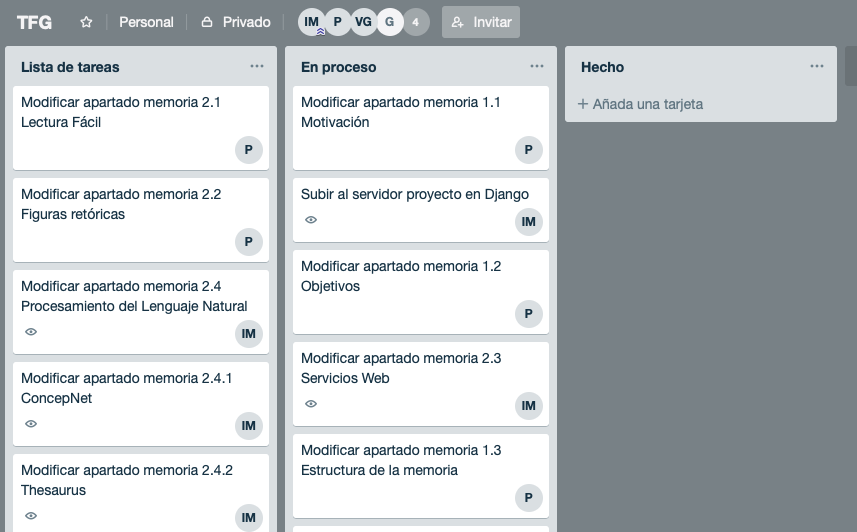
\includegraphics[width=1.0\textwidth]{Imagenes/Bitmap/Capitulo1/trello.png}
	\caption{Tablero de tareas al inicio del proyecto}
	\label{fig:trello}
\end{figure}


%-------------------------------------------------------------------
\section{Estructura de la memoria}
%-------------------------------------------------------------------
\label{cap:sec:estructuramemoria}


En el \textbf{capítulo dos} se presenta el Estado de la Cuestión, en el que se explicarán las redes semánticas: que son, que tipos existen y algunas herramientas que las implementan. Después, se explicará que es la lectura fácil y como se aplica y se hablará de las figuras retóricas. Por último se explicarán que son los servicios web, los tipos que existen, su arquitectura, y las ventajas y desventajas de su uso.

En el \textbf{capítulo tres} se explicarán las herramientas utilizadas para la creación de este trabajo, como pueden ser Django para el desarrollo de la aplicación y SpaCy para el etiquetado de palabras. Se describirá para que se utilizan estas herramientas y sus características principales.

En el \textbf{capítulo cuatro} se explicará todo lo relacionado con la aplicación. Su diseño, la implementación donde se explicará su arquitectura, como está diseñada la base de datos, que red semántica se utilizó, el backend y el frontend. Por último se describirá la evaluación realizada con expertos.

 
En el \textbf{capítulo cinco} se describe el trabajo realizado por cada uno de los autores de dicho proyecto.

En el \textbf{capítulo seis} se detallan las conclusiones obtenidas tras la finalización del proyecto así como el trabajo futuro que se podría realizar.